\def\us{\char`\_}

\documentclass[a4paper, 12pt]{article}
%\documentclass{article}

\usepackage{fullpage}
\usepackage{pgf}
\usepackage{tikz}
\usetikzlibrary{arrows,automata,shapes}
\usepackage{multirow}
\usepackage{color}
\usepackage[latin1]{inputenc}
\usepackage{verbatim}
\usepackage{amsmath}
\usepackage{times,mathptmx}
\usepackage{chngcntr}
\usepackage{hyperref}
\usepackage{enumitem}
\usepackage{scrextend}
%\usepackage[table]{xcolor}
\usepackage{listings}
\definecolor{light-gray}{gray}{0.95}
%\usepackage[firstpage]{draftwatermark}


\usepackage{listings}
\usepackage{cancel}
\graphicspath{ {../../../../figures/} }

\newenvironment{packed_enum}{
\begin{itemize}[leftmargin=0pt,topsep=-12pt]
	\setlength{\itemsep}{1pt}
	\setlength{\parskip}{0pt}
	\setlength{\parsep}{0pt}
}{\end{itemize}}

\newenvironment{packed_items}{
\begin{itemize}[topsep=-12pt]
	\setlength{\itemsep}{1pt}
	\setlength{\parskip}{0pt}
	\setlength{\parsep}{0pt}
}{\end{itemize}}


%%%%%%%%%%%%%%%%%%%%%%%%%%%%%%%%%%%%%%%%%%%%%%%%%%%%%%%%%%%%%%%%%%%%%%%%%%%
% creating subsubsubsection notation
% src: http://www.latex-community.org/forum/viewtopic.php?f=5&t=791
%%%%%%%%%%%%%%%%%%%%%%%%%%%%%%%%%%%%%%%%%%%%%%%%%%%%%%%%%%%%%%%%%%%%%%%%%%%
\setcounter{secnumdepth}{6}
\renewcommand\theparagraph{\Alph{paragraph}}

\makeatletter
\renewcommand\paragraph{\@startsection{paragraph}{4}{\z@}%
                                     {-3.25ex\@plus -1ex \@minus -.2ex}%
                                     {0.0001pt \@plus .2ex}%
                                     {\normalfont\normalsize\bfseries}}
\renewcommand\subparagraph{\@startsection{subparagraph}{5}{\z@}%
                                     {-3.25ex\@plus -1ex \@minus -.2ex}%
                                     {0.0001pt \@plus .2ex}%
                                     {\normalfont\normalsize\bfseries}}
\counterwithin{paragraph}{subsubsection}
\counterwithin{subparagraph}{paragraph}
\makeatother
%%%%%%%%%%%%%%%%%%%%%%%%%%%%%%%%%%%%%%%%%%%%%%%%%%%%%%%%%%%%%%%%%%%%%%%%%%%%%%%%

\newcommand{\eqoffset}[1]{%
  {\ensuremath{%
      {\text{offset}}_{#1}}%
  }%
}
\newcommand{\eqdelay}[1]{{\text{delay}}_{#1}}
\newcommand{\eqasymm}{{\text{asymmetry}}}

\begin{document}

\title{White Rabbit Switch: Failures and Diagnostics}
\author{Grzegorz Daniluk\\ Adam Wujek\\[.5cm] CERN BE-CO-HT}
\maketitle
\thispagestyle{empty}

\begin{figure}[ht!]
  \centering
  \vspace{1.3cm}
  
\includegraphics[width=0.50\textwidth]{../images/WRlogo.pdf}
\end{figure}

\newpage

\newpage

\newpage

\tableofcontents

\newpage
\section{Introduction}

This document tries to list all possible ways the White Rabbit Switch can
break and describes the information exported from our device to help diagnose
the problems.

The document is organized in two parts. First one (section \ref{sec:failures})
tries to list all the possible failures that may disturb synchronization and
Ethernet switching. The structure of each failure description is the following:
\begin{itemize}[leftmargin=0pt]
	\item [] \underline{Mode}: for timing failures, it says which modes are
		affected. Possible values are:
		\begin{itemize}
			\item \emph{Slave} - WR Switch has at least one Slave port synchronized to
				another WR device higher in the timing hierarchy (though it may be also
				Master to other WR/PTP devices lower in the timing hierarchy).
			\item \emph{Grand Master} - WR Switch at the top of the synchronization
				hierarchy. It is synchronized to an external clock (e.g. GPSDO, Cesium)
				and provides timing to other WR/PTP devices.
			\item \emph{Free-Running Master} - WR Switch at the top of the
				synchronization hierarchy. It provides timing to other WR/PTP devices
				but runs from a local oscillator (not synchronized to external atomic
				clock).
		\end{itemize}

	\item [] \underline{Description}: What the problem is about, how important it
		is and what bad may happen if it occurs.
	\item [] \underline{SNMP objects}: Which SNMP objects should be monitored to
		detect the failure. These may be objects from \texttt{WR-SWITCH-MIB} or one
		of the standard MIBs used by the \emph{net-snmp}.
	\item [] \underline{Notes}: Optional comment for SNMP implementation. It may describe current
		implementation of ideas how to implement it in the future
\end{itemize}

Section \ref{sec:snmp_exports} is a documentation for people integrating WR
switch into a control system, operators and WR experts. It describes all
essential SNMP objects exported by the device divided into two groups:
\emph{Operator/basic objects}, \emph{Expert objects}


\newpage
\section{Possible Errors}
\label{sec:failures}
\subsection{Timing error}
As a timing error we define WR Switch not being able to provide its slave
nodes/switches with correct timing information consistent with the rest of the
WR network.\\

\noindent Faults leading to a timing error:
\begin{enumerate}
	\item {\bf \emph{PTP/PPSi} went out of \texttt{TRACK\_PHASE}}
		\label{fail:timing:ppsi_track_phase}
		\begin{packed_enum}
			\item [] \underline{Status}: DONE
			\item [] \underline{Severity}: ERROR
			\item [] \underline{Mode}: \emph{Slave}
			\item [] \underline{Description}:\\
				If \emph{PTP/PPSi} WR servo goes out of the \texttt{TRACK\_PHASE} state,
				that means something bad has happened and switch has lost the
				synchronization to its Master.
			\item [] \underline{SNMP objects}:\\
				\texttt{WR-SWITCH-MIB::wrsPtpServoState.<n>} - PTP servo state as string\\
				\texttt{WR-SWITCH-MIB::wrsPtpServoStateN.<n>} - PTP servo state as number
			\item [] \underline{Note}: PTP servo state is exported as a string and a number.
		\end{packed_enum}

	\item {\bf Offset jump not compensated by Slave}
		\label{fail:timing:offset_jump}
		\begin{packed_enum}
			\item [] \underline{Status}: DONE
			\item [] \underline{Severity}: ERROR
			\item [] \underline{Mode}: \emph{Slave}
			\item [] \underline{Description}:\\
				This may happen if Master resets its WR time counters (e.g. because it
				lost the link to its Master higher in the hierarchy or to external
				clock), but Slave switch does not follow the jump.
			\item [] \underline{SNMP objects}:\\
				\texttt{WR-SWITCH-MIB::wrsPtpClockOffsetPs.<n>} - value of the offset in ps\\
				\texttt{WR-SWITCH-MIB::wrsPtpClockOffsetPsHR.<n>} - 32-bit signed value of the offset in ps; with
				saturation on overflow and underflow
		\end{packed_enum}

	\item {\bf Detected jump in the RTT value calculated by \emph{PTP/PPSi}}
		\label{fail:timing:rtt_jump}
		\begin{packed_enum}
			\item [] \underline{Status}: DONE
			\item [] \underline{Severity}: ERROR
			\item [] \underline{Mode}: \emph{Slave}
			\item [] \underline{Description}:\\
				Once WR link is established round-trip delay (RTT) can change smoothly
				due to the temperature variations. If a sudden jump is detected, that
				means erroneous timestamp was generated either on Master or Slave side.
				One cause of that could be the wrong value of the t24p transition point.
			\item [] \underline{SNMP objects}:\\
				\texttt{WR-SWITCH-MIB::wrsPtpRTT.<n>}
			\item [] \underline{Note}: we  monitor RTT variations inside
				the switch to build up the general WRS status word (section XXX).
		\end{packed_enum}

	\item {\bf Wrong $\Delta_{TXM}$, $\Delta_{RXM}$, $\Delta_{TXS}$,
		$\Delta_{RXS}$ values are reported to the \emph{PTP/PPSi} daemon}
		\label{fail:timing:deltas_report}
		\begin{packed_enum}
			\item [] \underline{Status}: DONE
			\item [] \underline{Severity}: ERROR
			\item [] \underline{Mode}: \emph{all}
			\item [] \underline{Description}:\\
				If \emph{PTP/PPSi} doesn't get the correct values of fixed hardware delays,
				it won't be able to calculate a proper Master-to-Slave delay. Although
				the estimated offset in \emph{PTP/PPSi} is close to 0, WRS won't be
				synchronized to Master with the sub-nanosecond accuracy.
			\item [] \underline{SNMP objects}:\\
				\texttt{WR-SWITCH-MIB::wrsPtpDeltaTxM.<n>}\\
				\texttt{WR-SWITCH-MIB::wrsPtpDeltaRxM.<n>}\\
				\texttt{WR-SWITCH-MIB::wrsPtpDeltaTxS.<n>}\\
				\texttt{WR-SWITCH-MIB::wrsPtpDeltaRxS.<n>}
		\end{packed_enum}

	\item {\bf \emph{SoftPLL} became unlocked}
		\label{fail:timing:spll_unlock}
		\begin{packed_enum}
			\item [] \underline{Status}: DONE
			\item [] \underline{Severity}: ERROR
			\item [] \underline{Mode}: \emph{all}
			\item [] \underline{Description}:\\
				If \emph{SoftPLL} loses lock, for any reason, Slave or Grand Master
				switch can no longer be syntonized and phase aligned with its time
				source. WRS in Free-running mode without properly locked Helper PLL is
				not able to perform reliable phase measurements for enhancing Rx
				timestamps resolution. For Grand Master the reason of \emph{SoftPLL}
				going out of lock might be disconnected 1-PPS/10MHz signals or external
				clock down. In that case, the switch goes into Free-running mode and
				resets WR time. Later we will have a holdover to keep the Grand Master
				switch disciplined in case it loses external reference.
			\item [] \underline{SNMP objects}:\\
				\texttt{WR-SWITCH-MIB::wrsSpllMode}\\
				\texttt{WR-SWITCH-MIB::wrsSpllSeqState}\\
				\texttt{WR-SWITCH-MIB::wrsSpllAlignState}\\
				\texttt{WR-SWITCH-MIB::wrsSpllHlock}\\
				\texttt{WR-SWITCH-MIB::wrsSpllMlock}\\
				\texttt{WR-SWITCH-MIB::wrsSpllDelCnt}
		\end{packed_enum}

	\item {\bf \emph{SoftPLL} has crashed/restarted}
		\label{fail:timing:spll_crash}
		\begin{packed_enum}
			\item [] \underline{Status}: TODO \emph{(depends on SoftPLL mem read), (require changes in lm32 software)}
			\item [] \underline{Severity}: ERROR
			\item [] \underline{Mode}: \emph{all}
			\item [] \underline{Description}:\\
				If LM32 software crashes or restarts for some reason, its state may be
				either reseted or random (if for some reason variables were overwritten
				with junk values). In such case PLL becomes unlocked and switch is not
				able to provide synchronization to other devices.
			\item [] \underline{SNMP objects}:\\
				\texttt{WR-SWITCH-MIB::wrsSpllIrqCnt}\\
				\texttt{WR-SWITCH-MIB::wrsStartCntSPLL} \emph{(not yet implemented)}
			\item [] \underline{Note}: We have a similar mechanism as in the
				\emph{wrpc-sw} to detect if the LM32 program has restarted because of
				the CPU following a NULL pointer. However, LM32 program hangs on
				re-initialization phase. 
				In addition to that, we can detect if
				\emph{SoftPLL} is hanging (but not restarted) based on irq counter.
		\end{packed_enum}

	\item {\bf Link to WR Master is down}
		\label{fail:timing:master_down}
		\begin{packed_enum}
			\item [] \underline{Status}: DONE
			\item [] \underline{Severity}: ERROR (will become WARNING with the
				switch-over)
			\item [] \underline{Mode}: \emph{Slave}
			\item [] \underline{Description}:\\
				In that case, WR Switch loses timing reference, resets counters
				responsible for keeping the WR time, and starts operating in a
				Free-Running Master mode.
			\item [] \underline{SNMP objects}:\\
				\texttt{WR-SWITCH-MIB::wrsPortStatusLink.<n>}\\
				\texttt{WR-SWITCH-MIB::wrsPortStatusConfiguredMode.<n>}
		\end{packed_enum}

	\item {\bf PTP frames don't reach ARM}
		\label{fail:timing:no_frames}
		\begin{packed_enum}
			\item [] \underline{Status}: TODO \emph{(depends on ppsi shm?)}
			\item [] \underline{Severity}: ERROR
			\item [] \underline{Mode}: \emph{all}
			\item [] \underline{Description}:\\
				In this case, \emph{PTP/PPSi} will fail to stay synchronized and provide
				synchronization. Even if WR servo is in the \texttt{TRACK\_PHASE} state,
				it calculates new phase shift based on the Master-to-Slave delay
				variations. To calculate these variations, it still needs timestamped
				PTP frames flowing. There could be several causes of such fault:
				\begin{itemize}
					\item HDL problem (e.g. SwCore or Endpoint hanging)
					\item \emph{wr\_nic.ko} driver crash
					\item wrong VLANs configuration
				\end{itemize}
			\item [] \underline{SNMP objects}:\\
				\texttt{WR-SWITCH-MIB::wrsPortStatusPtpTxFrames.<n>}\\
				\texttt{WR-SWITCH-MIB::wrsPortStatusPtpRxFrames.<n>}\\
				\texttt{WR-SWITCH-MIB::wrsPortStatusLink.<n>}\\
				\texttt{WR-SWITCH-MIB::wrsPortStatusConfiguredMode.<n>}
			\item [] \underline{Note}: If the kernel driver crashes, there is not much
				we can do. We end up with either our system frozen or a reboot. For
				wrong VLAN configuration and HDL problems we can monitor if PTP frames
				are flowing on Slave port(s) of WRS and raise an alarm (change status
				word) if they don't flow anymore. We should combine this with the link
				status (up/down). If VLANs are misconfigured, we don't receive PTP
				frames, but the link is still up. This could let us distinguish from a
				lack of frames due to the link down (which is a separate issue).
		\end{packed_enum}

	\item {\bf Detected SFP not supported for WR timing}
		\label{fail:timing:wrong_sfp}
		\begin{packed_enum}
			\item [] \underline{Status}: DONE
			\item [] \underline{Severity}: ERROR
			\item [] \underline{Mode}: \emph{all}
			\item [] \underline{Description}:\\
				By not supported SFP for WR timing we mean a transceiver that doesn't
				have the \emph{alpha} parameter and fixed hardware delays defined in the
				SFP database (\texttt{CONFIG\_SFPXX\_PARAMS} parameters in dot-config). The consequence is
				\emph{PTP/PPSi} not having the right values to estimate link asymmetry.
				Despite \emph{PTP/PPSi} offset being close to 0 \emph{ps}, the device won't
				be properly synchronized.
			\item [] \underline{SNMP objects}:\\
				\texttt{WR-SWITCH-MIB::wrsPortStatusSfpVN.<n>}\\
				\texttt{WR-SWITCH-MIB::wrsPortStatusSfpPN.<n>}\\
				\texttt{WR-SWITCH-MIB::wrsPortStatusSfpVS.<n>}\\
				\texttt{WR-SWITCH-MIB::wrsPortStatusSfpInDB.<n>}\\
				\texttt{WR-SWITCH-MIB::wrsPortStatusSfpGbE.<n>}\\
				\texttt{WR-SWITCH-MIB::wrsPortStatusSfpError.<n>}
			\item [] \underline{Note}: WRS configuration allow to disable this check on some ports.
				That is because ports may be used for regular (non-WR) PTP
				synchronization or for data transfer only (no timing). In that case any
				Gigabit SFP can be used (also copper). Detecting if a non-Gigabit
				Ethernet SFP is plugged into the cage is covered in a separate issue
				\ref{fail:other:sfp} in section \ref{sec:other_fail}.
		\end{packed_enum}

	\item {\bf \emph{PTP/PPSi} process has crashed/restarted}
		\label{fail:timing:ppsi_crash}
		\begin{packed_enum}
			\item [] \underline{Status}: DONE
			\item [] \underline{Severity}: ERROR
			\item [] \underline{Mode}: \emph{all}
			\item [] \underline{Description}:\\
				If the \emph{PTP/PPSi} daemon crashes we lose any synchronization
				capabilities. Then \texttt{Monit} restarts missing process.
				Number of particular process starts is stored in corresponding object.
			\item [] \underline{SNMP objects}:\\
				\texttt{WR-SWITCH-MIB::wrsStartCntPTP}\\
				\texttt{WR-SWITCH-MIB::wrsBootUserspaceDaemonsMissing}\\
				\texttt{HOST-RESOURCES-MIB::hrSWRunName.<n>}
		\end{packed_enum}

	\item {\bf \emph{HAL} process has crashed/restarted}
		\label{fail:timing:hal_crash}
		\begin{packed_enum}
			\item [] \underline{Status}: DONE
			\item [] \underline{Severity}: WARNING (but only after we modify PTP/PPSi so
				it reconnects to HAL, and HAL does not re-initialize SoftPLL after
				crash)
			\item [] \underline{Mode}: \emph{all}
			\item [] \underline{Description}:\\
				If \emph{HAL} crashes, \emph{PTP/PPSi} is not able to communicate with
				hardware i.e. read phase shift, get timestamps, phase shift the clock
				etc. When \emph{HAL} crashes then \texttt{Monit} will restart it.
			\item [] \underline{SNMP objects}:\\
				\texttt{WR-SWITCH-MIB::wrsStartCntHAL}\\
				\texttt{WR-SWITCH-MIB::wrsBootUserspaceDaemonsMissing}\\
				\texttt{HOST-RESOURCES-MIB::hrSWRunName.<n>}
		\end{packed_enum}

	\item {\bf Wrong configuration applied}
		\label{fail:timing:wrong_config}
		\begin{packed_enum}
			\item [] \underline{Status}: TODO \emph{(to be done later)}
			\item [] \underline{Severity}: WARNING
			\item [] \underline{Mode}: \emph{all}
			\item [] \underline{Description}:\\
				If there is a wrong configuration applied to the \emph{PTP/PPSi} or HAL
				(i.e.  wrong fixed delays, mode of operation etc.) there is not much we
				can do. The responsibility of WR experts (or person deploying the
				system) is to make sure that all the devices have correct initial
				configuration. Later we can only generate warnings, if the key
				configuration options are changed remotely (e.g. Grand Master mode to
				Free-running Master or updated fixed hardware delays values).\\
				For misconfigured VLANs, we can monitor if PTP frames are flowing on
				Slave port(s) of the switch.
			\item [] \underline{SNMP objects}: \emph{(not yet implemented)}
			\item [] \underline{Note}: monitor remote updates of key configuration
				options (PTP/WR mode, fixed hardware delays)
		\end{packed_enum}

	\item {\bf Switchover failed}
		\begin{packed_enum}
			\item [] \underline{Status}: for later
			\item [] \underline{Severity}: ERROR
			\item [] \underline{Mode}: \emph{Slave}, \emph{Grand Master}
			\item [] \underline{Description}: \emph{(not yet implemented)}\\
				In case the primary timing link breaks, switchover is responsible for
				seamless switching to the backup one to keep the device in sync. If WRS
				operates in a \emph{Slave} mode, switchover is about switching
				between two (or more) WR links to one or multiple WR Masters. If it
				operates in a \emph{Grand Master} mode, it is about broken/lost
				connection to an external reference and switching to a backup WR link
				(another WR Master). Regardless of the configuration, if we fail to
				switch-over to a backup link (e.g. because the it is down), WRS resets
				the time counters and continue the operation as a Free-Running Master.
			\item [] \underline{SNMP objects}: \emph{(not yet implemented)}
			\item [] \underline{Note}: we should probably use parameters reported by
				the backup channel(s) of the SoftPLL and the backup PTP servo to be able
				to detect and report that something went wrong.
		\end{packed_enum}

	\item {\bf Holdover for too long}
		\begin{packed_enum}
			\item [] \underline{Status}: for later
			\item [] \underline{Severity}: WARNING
			\item [] \underline{Mode}: \emph{Grand Master}
			\item [] \underline{Description}: \emph{(not yet implemented)}\\
				Signaling active holdover is one thing, but if a Grand Master switch is
				kept in sync with holdover for too long, it might drift away from the
				ideal external reference too much. All devices in WR network will be
				still synchronized, but no longer in sync with external reference.
			\item [] \underline{SNMP objects}: \emph{(not yet implemented)}
		\end{packed_enum}

\end{enumerate}

\newpage
\subsection{Data error}
As a data error we define WR Switch not being able to forward Ethernet traffic
between devices connected to the ports.\\

\noindent Faults leading to a data error:
\begin{enumerate}

	\item {\bf Link down}
		\label{fail:data:link_down}
		\begin{packed_enum}
			\item [] \underline{Status}: DONE  \emph{(to be changed later for switchover)}
			\item [] \underline{Severity}: ERROR (will be WARNING with the
				switch-over)
			\item [] \underline{Description}:\\
				This obviously stops the flow of frames on an Ethernet port and there is
				not much we can do besides reporting an error. Topology redundancy is a
				cure for that (if backup link is fine, and reconfiguration does not
				fail). There might be several causes of a link down:
				\begin{itemize}
					\item unplugged fiber
					\item broken fiber
					\item broken SFP
					\item wrong(non-complementary) pair of WDM SPFs is used
				\end{itemize}
				However, we are not able to distinguish between them inside the switch.
			\item [] \underline{SNMP objects}:\\
				\texttt{IF-MIB::ifOperStatus.<n>}\\
				\texttt{WR-SWITCH-MIB::wrsPortStatusLink.<n>}
		\end{packed_enum}

	\item {\bf Fault in the Endpoint's transmission/reception path}
		\label{fail:data:ep_txrx}
		\begin{packed_enum}
			\item [] \underline{Status}: DONE
			\item [] \underline{Severity}: ERROR
			\item [] \underline{Description}:\\
				This fault covers various errors reported by the Endpoint, e.g. FIFO
				underrun in the Tx PCS or FIFO overrun in the Rx PCS, receiving invalid
				\emph{8b10b} code, CRC error etc.
			\item [] \underline{SNMP objects}:\\
				\texttt{WR-SWITCH-MIB::wrsPstatsTXUnderrun.<n>}\\
				\texttt{WR-SWITCH-MIB::wrsPstatsRXOverrun.<n>}\\
				\texttt{WR-SWITCH-MIB::wrsPstatsRXInvalidCode.<n>}\\
				\texttt{WR-SWITCH-MIB::wrsPstatsRXSyncLost.<n>}\\
				\texttt{WR-SWITCH-MIB::wrsPstatsRXPfilterDropped.<n>}\\
				\texttt{WR-SWITCH-MIB::wrsPstatsRXPCSErrors.<n>}\\
				\texttt{WR-SWITCH-MIB::wrsPstatsRXCRCErrors.<n>}
		\end{packed_enum}

	\item {\bf Problem with the \emph{SwCore} or Endpoint HDL module}
		\label{fail:data:swcore_hang}
		\begin{packed_enum}
			\item [] \underline{Status}: TODO \emph{(depends on HDL, then hal?)}
			\item [] \underline{Severity}: ERROR
			\item [] \underline{Description}:\\
				If any of these HDL modules hangs, there is usually not much the user
				can do besides resetting the WR Switch so that the FPGA is reprogrammed.
				It may happen that frames are lost only on one or two ports, but it may
				be also that the whole SwCore refuses to forward traffic.
			\item [] \underline{SNMP objects}:\\
				\texttt{WR-SWITCH-MIB::wrsPstatsTXFrames.<n>}\\
				\texttt{WR-SWITCH-MIB::wrsPstatsForwarded.<n>}
			\item [] \underline{Note}: We should probably provide also some events for
				counting from the SwCore.\\
				Two early ideas for checking if SwCore is hanging or not:
				\begin{itemize}
					\item Monitor the number of used and free pages in the MPM memory
					\item Compare per-port \emph{RTUfwd} counter with the \emph{Tx}
						Endpoint counter for this port. \emph{RTUfwd} counts all forwarding
						decisions from RTU to the port $<$n$>$ (including PTP frames from
						NIC). If this number is equal to the number of frames actually
						transmitted by the Endpoint, then everything works fine).
				\end{itemize}
		\end{packed_enum}

	\item {\bf RTU is full and cannot accept more requests}
		\label{fail:data:rtu_full}
		\begin{packed_enum}
			\item [] \underline{Status}: DONE
			\item [] \underline{Severity}: ERROR
			\item [] \underline{Description}:\\
				If RTU is full for a given port, it's not able to accept more requests
				and generate new responses. In such case frames are dropped in the
				Rx path of the Endpoint.
			\item [] \underline{SNMP objects}:\\
				\texttt{WR-SWITCh-MIB::wrsPstatsRXDropRTUFull.<n>}
		\end{packed_enum}

	\item {\bf Too much HP traffic / Per-priority queue full}
		\label{fail:data:too_much_HP}
		\begin{packed_enum}
			\item [] \underline{Status}: TODO \emph{(depends on HDL)}
			\item [] \underline{Severity}: ERROR
			\item [] \underline{Description}:\\
				If we get too much High Priority traffic, then SwCore will be busy all
				the time forwarding HP frames. This way regular/best effort traffic
				won't be flowing through the switch. In the extreme case, HP traffic
				queue may become full and we start losing HP frames, which is
				unacceptable.
			\item [] \underline{SNMP objects}:\\
				\texttt{WR-SWITCH-MIB::wrsPstatsFastMatchPriority.<n>} - HP frames on a port\\
				\texttt{WR-SWITCH-MIB::wrsPstatsRXFrames<n>} - Total number of Rx frames on
				the port\\
				\texttt{WR-SWITCh-MIB::wrsPstatsRXPrio0.<n>} - Rx priorities 0-7\\
				\texttt{[..]}\\
				\texttt{WR-SWITCh-MIB::wrsPstatsRXPrio7.<n>}
			\item [] \underline{Note}: we need to get from SwCore the information
				about per-priority queue utilization, or at least an event when it's
				full.
		\end{packed_enum}

	\item {\bf \emph{RTUd} has crashed}
		\label{fail:data:rtu_crash}
		\begin{packed_enum}
			\item [] \underline{Status}: DONE
			\item [] \underline{Severity}: WARNING
			\item [] \underline{Description}:\\
				If \emph{RTUd} crashed, traffic would be still routed between the WRS ports, but
				only based on already existing static and dynamic rules. There would be
				no learning or aging functionality. That means MAC addresses wouldn't be
				removed from the RTU table if a device is disconnected from port. Since
				there would be no learning, each frame with yet unknown destination MAC
				will be broadcast to all ports (within a VLAN).
				When \emph{RTUd} crashes then \texttt{Monit} will restart it.
			\item [] \underline{SNMP objects}:\\
				\texttt{WR-SWITCH-MIB::wrsStartCntRTUd}\\
				\texttt{WR-SWITCH-MIB::wrsBootUserspaceDaemonsMissing}\\
				\texttt{HOST-RESOURCES-MIB::hrSWRunName.<n>} \emph{(implemented)}
		\end{packed_enum}

	\item {\bf Network loop - two or more identical MACs on two or more ports}
		\label{fail:data:net_loop}
		\begin{packed_enum}
			\item [] \underline{Status}: TODO \emph{(to be done later)}
			\item [] \underline{Severity}: ERROR
			\item [] \underline{Description}:\\
				In such case we have a ping-pong situation. If two ports receive frames
				with the same source MAC, it is learned on one of these ports. Then if
				it comes on a second port, it is learned on a second port, and removed
				from the first one. Later, MAC is learned again on the first port, and
				removed from the MAC table for the second port, and so on. This
				situation is a network configuration problem or eRSTP failure.
			\item [] \underline{SNMP objects}: \emph{(not yet implemented)}
			\item [] \underline{Note}: we need to monitor the \emph{rtu\_stat} to
				diagnose ping-pong in the RTU table.
		\end{packed_enum}

	\item {\bf Wrong configuration applied (e.g. wrong VLAN config)}
		\begin{packed_enum}
			\item [] \underline{Status}: TODO \emph{(to be done later)}
			\item [] \underline{Severity}: WARNING
			\item [] \underline{Description}:\\
				The same problem as described in the timing fault
				\ref{fail:timing:no_frames}
		\end{packed_enum}

	\item {\bf Topology Redundancy failure}
		\begin{packed_enum}
			\item [] \underline{Status}: for later
			\item [] \underline{Severity}: ERROR
			\item [] \underline{Description}: \emph{(not yet implemented)}\\
				Topology redundancy let's us prevent from losing data when the primary
				uplink is down for some reason. However, if a backup link is also down
				or reconfiguration to backup link fails, we start losing data and an
				alarm should be raised.
			\item [] \underline{SNMP objects}: \emph{(not yet implemented)}
			\item [] \underline{Note}: One thing we need to report is a backup link(s)
				going down, but we should also think about how to determine if there is
				some problem with eRSTP and if it may fail/has failed if the primary
				link is down.
		\end{packed_enum}

\end{enumerate}

\newpage
\subsection{Other errors}
\label{sec:other_fail}

\begin{enumerate}
	\item {\bf WR Switch did not boot correctly}
		\label{fail:other:boot}
		\begin{packed_enum}
			\item [] \underline{Status}: QUESTION, TODO (add stop restarting system after defined number of restarts)
			\item [] \underline{Severity}: ERROR
			\item [] \underline{Description}:\\
				That one is about making sure that everything is up and running after WR
				switch boots. If any of the services fails, an alarm should be raised.
			\item [] \underline{SNMP objects}:\\
				\texttt{WR-SWITCH-MIB::wrsBootSuccessful} - status word informing whether switch booted correctly\\
				\texttt{WR-SWITCH-MIB::wrsBootHwinfoReadout}\\
				\texttt{WR-SWITCH-MIB::wrsBootLoadFPGA}\\
				\texttt{WR-SWITCH-MIB::wrsBootLoadLM32}\\
				\texttt{WR-SWITCH-MIB::wrsBootKernelModulesMissing}\\
				\texttt{WR-SWITCH-MIB::wrsBootUserspaceDaemonsMissing}
			\item [] \underline{!QUESTION!}: \\
				Shall we stop restarting system after XXX restarts? Maybe dot-config option?
			\item [] \underline{Note}: we should have a flag somewhere reported
				through the SNMP (e.g. in the main status word) saying that WRS has
				booted correctly, FPGA is programmed, all kernel drivers are loaded and
				all daemons are up and running. If it's not the case, we should report
				what has happened:
				\begin{itemize}
					\item reading HW information from dataflash failed ?
					\item programming FPGA or LM32 failed ?
					\item loading any of the kernel modules failed ?
					\item starting any of the userspace daemons failed ?
				\end{itemize}
				The idea for that is to reboot the system if it was not able to boot
				correctly. Then we use the scratchpad registers of the processor to keep
				the boot count. If the value of this counter is more than X we stop
				rebooting and try to have a system running with at least \emph{dropbear}
				for SSH and \emph{net-snmp} to allow remote diagnostics. If on the other
				hand we have booted correctly we set the boot count to 0.
		\end{packed_enum}

	\item {\bf dot-config error}
		\label{fail:other:dot-config}
		\begin{packed_enum}
			\item [] \underline{Status}: DONE
			\item [] \underline{Severity}: ERROR
			\item [] \underline{Description}:\\
				Dot-config file used to configure switch can be stored locally or retreived from the network.
				Notify about source of dot-config and result of its downloading and veryfying.
			\item [] \underline{SNMP objects}:\\
				\texttt{WR-SWITCH-MIB::wrsBootSuccessful} - status word informing whether switch booted correctly\\
				\texttt{WR-SWITCH-MIB::wrsConfigSource} - source of dot-config, local or protocol which was used do download dot-config\\
				\texttt{WR-SWITCH-MIB::wrsConfigSourceHost} - address of server providing dot-config if non local\\
				\texttt{WR-SWITCH-MIB::wrsConfigSourceFilename} - path on a server to dot-config if non local\\
				\texttt{WR-SWITCH-MIB::wrsBootConfigStatus} - result of veryfication of dot-config
		\end{packed_enum}

	\item {\bf Any userspace daemon has crashed/restarted}
		\label{fail:other:daemon_crash}
		\begin{packed_enum}
			\item [] \underline{Status}: QUESTION, TODO \emph{(depends on monit)}
			\item [] \underline{Severity}: ERROR / WARNING (depending on the process)
			\item [] \underline{Description}:\\
				Running processes are monitored by \texttt{Monit}. When any of them crash,
				then \texttt{Monit} restarts missing process. If particular process is restarted
				5 times within 100 seconds then entire switch is restarted.
			\item [] \underline{SNMP objects}:\\
				\texttt{HOST-RESOURCES-MIB::hrSWRunName.<n>} - list of processes in standard MIB\\
				\texttt{WR-SWITCH-MIB::wrsStartCntHAL}\\
				\texttt{WR-SWITCH-MIB::wrsStartCntPTP}\\
				\texttt{WR-SWITCH-MIB::wrsStartCntRTUd}\\
				\texttt{WR-SWITCH-MIB::wrsStartCntSshd}\\
				\texttt{WR-SWITCH-MIB::wrsStartCntHttpd}\\
				\texttt{WR-SWITCH-MIB::wrsStartCntSnmpd}\\
				\texttt{WR-SWITCH-MIB::wrsStartCntSyslogd}\\
				\texttt{WR-SWITCH-MIB::wrsStartCntWrsWatchdog}\\
				\texttt{WR-SWITCH-MIB::wrsStartCntSPLL} \emph{(not implemented)}\\
				\texttt{WR-SWITCH-MIB::wrsBootUserspaceDaemonsMissing} - number of missing processes\\
				\texttt{WR-SWITCH-MIB::wrsBootSuccessful} - status word informing whether switch booted correctly
			\item [] \underline{!QUESTION!}: \\
				Shall we distinguish between crucial and less crucial processes? We don't do that now.
				We also don't warn in any special way about crashes other than increasing start counters.
			\item [] \underline{Note}: We have to monitor the list of running
				processes and their PIDs. We shall distinguish between crucial
				processes - error should be reported if one of them crashes; and less
				important processes which should just be restarted if they crash (and
				warning should be reported). If any of the processes has crashed, we
				need to restart it and increment a per-process counter reported through
				the SNMP to indicate how many times each process has crashed.\\

				Crucial processes (Error report if any of them crashes):
				\begin{itemize}
					\item \emph{PTP/PPSi}
					\item \emph{WRSW\_RTUd} - after adding configuration preserving code
						on restart, RTUd could be crossed out from this list
					\item \emph{WRSW\_HAL}
				\end{itemize}
				Less critical processes (Restarting them and Warning generation is
				enough):
				\begin{itemize}
					\item \emph{dropbear}
					\item \emph{udhcpc}
					\item \emph{rsyslogd}
					\item \emph{snmpd}
					\item \emph{lighttpd}
					\item \emph{TRUd/eRSTPd} - not yet implemented
				\end{itemize}

				\emph{RTUd} - we need to set the flag that it has crashed so that when
				it runs again it knows that HDL is already configured. It should not
				erase static entries in RTU table (e.g. multicasts for PTP) and it
				should not erase or it should configure again static entries set by-hand
				as well as VLANs. Dynamic entries are not a problem. RTUd will learn all
				MACs after restarting. The only consequence will be increased network
				traffic due to frames broadcast until all MACs are learned. In general
				the source code has to be checked to make sure what is cleared on
				startup and modified to preserve the configuration.\\

				\emph{TRUd/eRSTPd} - topology reconfiguration is done in hardware if
				needed, this daemon is used only to configure TRU/RTU HDL module.
				However, the story is similar as with the RTUd. If eRSTPd crashes, we
				need to store this information so that when it runs again, it does not
				erase the whole configuration. Also if topology reconfiguration is done
				in HDL while eRSTPd is down, HDL should keep the flag that it happened,
				and eRSTPd should read this flag when starting, so that it's aware that
				now, backup link is active.\\
		\end{packed_enum}

	\item {\bf Kernel crash}
		\begin{packed_enum}
			\item [] \underline{Status}: DONE
			\item [] \underline{Severity}: ERROR
			\item [] \underline{Description}:
				If Linux kernel has crashed the system reboots. Until next boot we have
				no synchronization, no SNMP to report the status, FPGA may be still
				forwarding Ethernet traffic, but based on dynamic and static routing
				rules from before the crash. Based on SNMP objects below it is possible
				to figure out that reboot took place and what was the reason for last reboot.
			\item [] \underline{SNMP objects}:\\
				\texttt{WR-SWITCH-MIB::wrsBootCnt}\\
				\texttt{WR-SWITCH-MIB::wrsRebootCnt}\\
				\texttt{WR-SWITCH-MIB::wrsRestartReason}\\
				\texttt{WR-SWITCH-MIB::wrsFaultIP} \emph{(not implemented)}\\
				\texttt{WR-SWITCH-MIB::wrsFaultLR} \emph{(not implemented)}
			\item [] \underline{Note}:
				Unfortunately it is not possible right now to distinguish whether reboot was caused by
				panic function of the kernel or the \texttt{reboot} command.
				Saving of IP and LR registers has to be implemented.
		\end{packed_enum}
	\item {\bf System nearly out of memory}
		\label{fail:other:no_mem}
		\begin{packed_enum}
			\item [] \underline{Status}: DONE
			\item [] \underline{Severity}: WARNING
			\item [] \underline{Description}:
				We need to monitor and report the amount of the
				free memory, report it through SNMP and raise an alarm if it's extremely
				low (but still enough to keep the system running).
			\item [] \underline{SNMP objects}:\\
				\texttt{WR-SWITCH-MIB::wrsMemoryTotal}\\
				\texttt{WR-SWITCH-MIB::wrsMemoryUsed}\\
				\texttt{WR-SWITCH-MIB::wrsMemoryUsedPerc} - percentage of used memory\\
				\texttt{WR-SWITCH-MIB::wrsMemoryFree}\\
				\texttt{WR-SWITCH-MIB::wrsMemoryFreeLow} - warn or error when low memory
		\end{packed_enum}
	\item {\bf Disk space low}
		\label{fail:other:no_disk}
		\begin{packed_enum}
			\item [] \underline{Status}: DONE
			\item [] \underline{Severity}: WARNING
			\item [] \underline{Description}:
				We need to monitor and report the amount of the
				free disk space, report it through SNMP and raise an alarm if it's extremely
				low (but still enough to keep the system running).
			\item [] \underline{SNMP objects}:\\
				\texttt{WR-SWITCH-MIB::wrsDiskMountPath.<n>}\\
				\texttt{WR-SWITCH-MIB::wrsDiskSize.<n>}\\
				\texttt{WR-SWITCH-MIB::wrsDiskUsed.<n>}\\
				\texttt{WR-SWITCH-MIB::wrsDiskFree.<n>}\\
				\texttt{WR-SWITCH-MIB::wrsDiskUseRate.<n>}\\
				\texttt{WR-SWITCH-MIB::wrsDiskFilesystem.<n>}\\
				\texttt{WR-SWITCH-MIB::wrsDiskSpaceLow} - warn or error when low disk space\\
				\texttt{HOST-RESOURCES-MIB::hrStorageDescr.<n>}\\
				\texttt{HOST-RESOURCES-MIB::hrStorageSize.<n>}\\
				\texttt{HOST-RESOURCES-MIB::hrStorageUsed.<n>}
			\item [] \underline{Note}:
				Objects like \texttt{HOST-RESOURCES-MIB::hrStorage*.<n>} are available via standard MIB.
				The same functionality is implemented in \texttt{WR-SWITCH-MIB}'s objects
				\texttt{wrsDisk*.<n>}
				(to ease implementation of \texttt{wrsDiskSpaceLow}).
		\end{packed_enum}

	\item {\bf CPU load too high}
		\label{fail:other:cpu}
		\begin{packed_enum}
			\item [] \underline{Status}: DONE
			\item [] \underline{Severity}: WARNING
			\item [] \underline{Description}:
				On a healthy swith CPU's load average shall be below 0.1. Some actions like
				SNMP queries or web interface acitvity may increase system's load average.
				System load average from 1, 5 and 15 minutes is exported via below objects.
				Additionaly \texttt{wrsCpuLoadHigh} warn or error on too high load.
			\item [] \underline{SNMP objects}:\\
				\texttt{WR-SWITCH-MIB::wrsCPULoadAvg1min}\\
				\texttt{WR-SWITCH-MIB::wrsCPULoadAvg5min}\\
				\texttt{WR-SWITCH-MIB::wrsCPULoadAvg15min}\\
				\texttt{WR-SWITCH-MIB::wrsCpuLoadHigh} - warn or error when CPU load too high
		\end{packed_enum}

	\item {\bf Temperature inside the box too high}
		\label{fail:other:temp}
		\begin{packed_enum}
			\item [] \underline{Status}: DONE
			\item [] \underline{Severity}: WARNING
			\item [] \underline{Description}:\\
				If the temperature raises too high we might break our electronics inside
				the box. It also means that most probably one or both of the fans inside
				the box are broken and should be replaced. There are 4 temperature
				sensors monitored:
				\begin{itemize}
					\item \emph{IC19} - temperature below the FPGA
					\item \emph{IC20}, \emph{IC17} - temperature near the SCB power supply
						circuit
					\item \emph{IC18} - temperature near the VCXO and PLLs (AD9516,
						CDCM6100)
				\end{itemize}
			\item [] \underline{SNMP objects}:\\
				\texttt{WR-SWITCH-MIB::wrsTempFPGA}\\
				\texttt{WR-SWITCH-MIB::wrsTempPLL}\\
				\texttt{WR-SWITCH-MIB::wrsTempPSL}\\
				\texttt{WR-SWITCH-MIB::wrsTempPSR}\\
				\texttt{WR-SWITCH-MIB::wrsTempThresholdFPGA}\\
				\texttt{WR-SWITCH-MIB::wrsTempThresholdPLL}\\
				\texttt{WR-SWITCH-MIB::wrsTempThresholdPSL}\\
				\texttt{WR-SWITCH-MIB::wrsTempThresholdPSR}\\
				\texttt{WR-SWITCH-MIB::wrsTemperatureWarning}
			\item [] \underline{Note}:
			\texttt{wrsTemperatureWarning} is raised when temperature read from any of these sensors
			exceeds individually set threshold in \emph{dot-config}. When at least one threshold
			temperature is not set tempWarning returns \emph{Threshold-not-set}.
			Temperature is read by the HAL to drive PWM inside the FPGA.
		\end{packed_enum}

	\item {\bf Not supported SFP plugged into the cage (especially non 1-Gb SFP)}
		\label{fail:other:sfp}
		\begin{packed_enum}
			\item [] \underline{Status}: DONE
			\item [] \underline{Severity}: WARNING
			\item [] \underline{Description}:\\
				If not supported Gigabit Fiber SFP is plugged into the cage, then it's a
				timing issue \ref{fail:timing:wrong_sfp}. However, if a non 1-Gb SFP is
				used, then no Ethernet traffic would be flowing on that port. It's due
				to the fact, that we don't have 10/100Mbit Ethernet implemented inside
				the WRS.
			\item [] \underline{SNMP objects}:\\
				\texttt{WR-SWITCH-MIB::wrsPortStatusSfpVN.<n>}\\
				\texttt{WR-SWITCH-MIB::wrsPortStatusSfpPN.<n>}\\
				\texttt{WR-SWITCH-MIB::wrsPortStatusSfpVS.<n>}\\
				\texttt{WR-SWITCH-MIB::wrsPortStatusSfpGbE.<n>}\\
				\texttt{WR-SWITCH-MIB::wrsPortStatusSfpError.<n>}\\
				\texttt{WR-SWITCH-MIB::wrsSFPsStatus} - status word for SFPs' status
		\end{packed_enum}

	\item {\bf File system / Memory corruption}
		\label{fail:other:memory}
		\begin{packed_enum}
			\item [] \underline{Description}:\\
			\item [] \underline{SNMP objects}: \emph{(none)}
			\item [] \underline{Note}: how shall we detect this ? Based on
				\emph{dmesg} errors reported by UBI and system in general ?\\
				This is bad, crazy things may happen, we can't do much about it.
		\end{packed_enum}

	\item {\bf Kernel freeze}
		\begin{packed_enum}
			\item [] \underline{Description}:
				If kernel freezes we can do nothing. It can freeze e.g. due to some
				infinite in the irq handler. It's like with the power failure, somebody
				has to go to the place where WRS is installed and investigate/restart
				the device.
			\item [] \underline{!QUESTION!}: Do we have watchdog in CPU? can we use it?
			\item [] \underline{SNMP objects}: \emph{(none)}
		\end{packed_enum}

	\item {\bf Power failure}
		\begin{packed_enum}
			\item [] \underline{Description}:\\
				Power failure may be either a WRS problem (i.e. broken power supply
				inside the switch) or an external problem (i.e. providing voltage to the
				device). There is not much reporting we can do in such case, it's up to
				the Network Management Station to raise an alarm if the SNMP Agent does
				not respond to the SNMP requests.
			\item [] \underline{SNMP objects}: \emph{(none)}
		\end{packed_enum}

	\item {\bf Hardware problem}
		\begin{packed_enum}
			\item [] \underline{Description}:\\
				If any crucial hardware part breaks we'll most probably notice it as one
				(or multiple) timing/data errors described in the previous sections.
				Besides that, we don't have any self-diagnostics on-board. Few examples:
				\begin{itemize}
					\item DAC / VCO - problems with synchronization
					\item cooling	fans - rise of the temperature inside the WRS box
						(failure \ref{fail:other:temp})
					\item power supply, ARM, FPGA - booting problem (failure
						\ref{fail:other:boot})
					\item memory chip - data corruption (failure \ref{fail:other:memory})
				\end{itemize}
			\item [] \underline{SNMP objects}: \emph{(none)}
		\end{packed_enum}

	\item {\bf Management link down}
		\label{fail:other:management_link}
		\begin{packed_enum}
			\item [] \underline{Description}:\\
				For obvious reasons we are not able to report through SNMP that the
				management link is down. This should be detected and reported by the NMS
				if it does not receive SNMP and ICMP responses from the WRS.
			\item [] \underline{SNMP objects}: \emph{(none)}
		\end{packed_enum}

	\item {\bf No static IP on the management port \& failed to DHCP}
		\begin{packed_enum}
			\item [] \underline{Description}:\\
				From operator's point of view it is similar to the issue
				\ref{fail:other:management_link}. WRS is not accessible through the
				management port, so its status cannot be reported. This should be
				detected and reported by the NMS if it does not receive SNMP and ICMP
				responses from the WRS. In such case WR expert should make a physical
				connection to the management USB port of the WRS to diagnose the
				problem.
			\item [] \underline{SNMP objects}: \emph{(none)}
		\end{packed_enum}

	\item {\bf IP address on the management port has changed}
		\begin{packed_enum}
			\item [] \underline{Status}: TODO
			\item [] \underline{Severity}: WARNING
			\item [] \underline{Description}:\\
				I'm not yet sure how we should report this. Probably SNMP is not the
				best choice because if the IP changes we're no longer able to poll SNMP
				objects (until IP is updated also in the Network Management Station). We
				should either generate SNMP trap to NMS or send Syslog message to a
				central server.
			\item [] \underline{SNMP objects}: \emph{(not yet implemented)}
		\end{packed_enum}

	\item {\bf Multiple unauthorized access attempts}
		\begin{packed_enum}
			\item [] \underline{Status}: for later
			\item [] \underline{Severity}: WARNING
			\item [] \underline{Description}:\\
				If we observe many attempts to gain a root access through ssh (or the
				web interface) that might mean somebody tries to do something nasty. We
				should report such situation as a Warning.
			\item [] \underline{SNMP objects}: \emph{(not yet implemented)}
			\item [] \underline{Note}: Bad password event is reported by syslog as
				warning. We should probably use this information to add an SNMP object.
		\end{packed_enum}

	\item {\bf Network reconfiguration (RSTP)}
		\label{fail:other:rstp}
		\begin{packed_enum}
			\item [] \underline{Status}: for later
			\item [] \underline{Severity}: WARNING
			\item [] \underline{Description}: \emph{(not yet implemented)}\\
				If topology reconfiguration occurs because of the primary link failure,
				this fact should be reported through SNMP as a warning. It's not
				critical situation, WR network still works. However, further
				investigation should be performed to repair the broken link.
			\item [] \underline{SNMP objects}: \emph{(not yet implemented)}
		\end{packed_enum}

	\item {\bf Backup link down}
		\begin{packed_enum}
			\item [] \underline{Status}: for later
			\item [] \underline{Severity}: WARNING
			\item [] \underline{Description}: \emph{(not yet implemented)}\\
				It's related to the issue \ref{fail:other:rstp}. If the WRS uses primary
				uplink, but the backup one fails, it's not a critical fault. WR Network
				still works, but the problem should be diagnosed and repaired to have
				the backup link operational in case the primary one fails.
			\item [] \underline{SNMP objects}: \emph{(not yet implemented)}
		\end{packed_enum}

\end{enumerate}

%\subsection{Switch out of sync to Master}
%
%\subsection{Switch made a big offset jump to follow Master}
%
%\subsection{Unsupported SFP plugged to one of the cages}
%
%\subsection{Lost lock to external 1-PPS \& 10 MHz}
%
%\subsection{Switch wasn't able to fetch initial time from NTP}
%
%\subsection{Suspicious value of any PTP parameter}
%e.g. bitslide > 16000;  dTx/dRx = 0, etc.
%
%\subsection{PPSi/HAL/SNMP/any other userspace daemon has crashed}
%
%\subsection{LM32 software has crashed/restarted}
%
%\subsection{Cooling fan broken}
%
%\subsection{Power supply broken}
%
%\subsection{Switch not reachable after power cut}
%
%\subsection{Switch not reachable through SNMP}
%
%\subsection{One of the links went down}
%
%\subsection{Ethernet frames being dumped}
%
%\subsection{Linux is out of memory}
%
%\subsection{Filesystem error/corruption}
%
%\subsection{HW version not recognized, FPGA bitstream not loaded}
%
%\subsection{Frames storm coming from one or multiple ports to CPU}

\newpage
\section{SNMP diagnostics and solving problems}
\label{sec:snmp_exports}
This section describes SNMP objects exported by the WR Switch. Objects within
the \texttt{WR\--SWITCH\--MIB} are divided into two groups:
\begin{itemize}
  \item General status objects for operators (section
    \ref{sec:snmp_exports:basic}) - provide a summary about the status of a
    switch and several main subsystems (like timing, networking, OS). These
    should be used by control system operators and users without a
    comprehensive knowledge of the White Rabbit internals. These exports provide
    a general status of the device and high level errors which is enough in most
    cases to perform a quick repair.

  \item Expert objects (section \ref{sec:snmp_exports:expert}) -
    can be used by White Rabbit experts for the in-depth diagnosis of the switch
    failures. These values are verbose and normally should not be used by the
    operators.
\end{itemize}

Description of the general status objects in section
\ref{sec:snmp_exports:basic} includes also a list of actions to follow if a
particular object reports an error. These repair procedures don't require any
in-depth knowledge about White Rabbit. Independently of an error reported, there
are some common remarks that apply to all situations:
\begin{itemize}
  \item Linux inside the WR Switch enumerates WR interfaces starting from 0.
    This means we have to use internally port indexes 0..17. However, the
    port numbers printed on the front panel are 1..18. Syslog messages
    generated from the switch use the Linux port numbering. The consequence is
    that every time Syslog says there is a problem on port X, this refers to
    port index X+1 on the front panel of the switch.
  \item If a procedure given for a specific SNMP object does not solve the
    problem. Please contact WR experts to perform more in-depth analysis of your
    network. For this, you should provide a complete dump of the WRS status
    generated in the first step of each procedure.
  \item First action in most of the procedures below named \emph{Dump state}
    requires simply calling a tool provided by WR developers that reads all the
    detailed information from the switch and writes it to a single file that can
    be later analyzed by the experts.\\
    {\bf TODO: point to the tool once it's done}
  \item If solving procedure requires restarting or replacing a broken WR
    Switch, please make sure that after the repair, all other WR devices
    connected to the affected switch are synchronized and do not report any
    problems.
  \item If a procedure requires replacing switch with a new unit, the broken one
    should be handled to WR experts or the switch manufacturer to investigate
    the problem.
\end{itemize}

\subsection{General status objects for operators}
\label{sec:snmp_exports:basic}
This section describes the general status MIB objects that represent the overall
status of a device and its subsystems. They are organized in a tree structure
(fig.\ref{fig:snmp_oper}) where each object reports a problem based on the
status of its child objects. SNMP object in the third layer of this tree are
calculated based on the SNMP expert objects. Most of the status objects
described in this section can have one of the following values:
\begin{figure}[ht]
  \begin{center}
    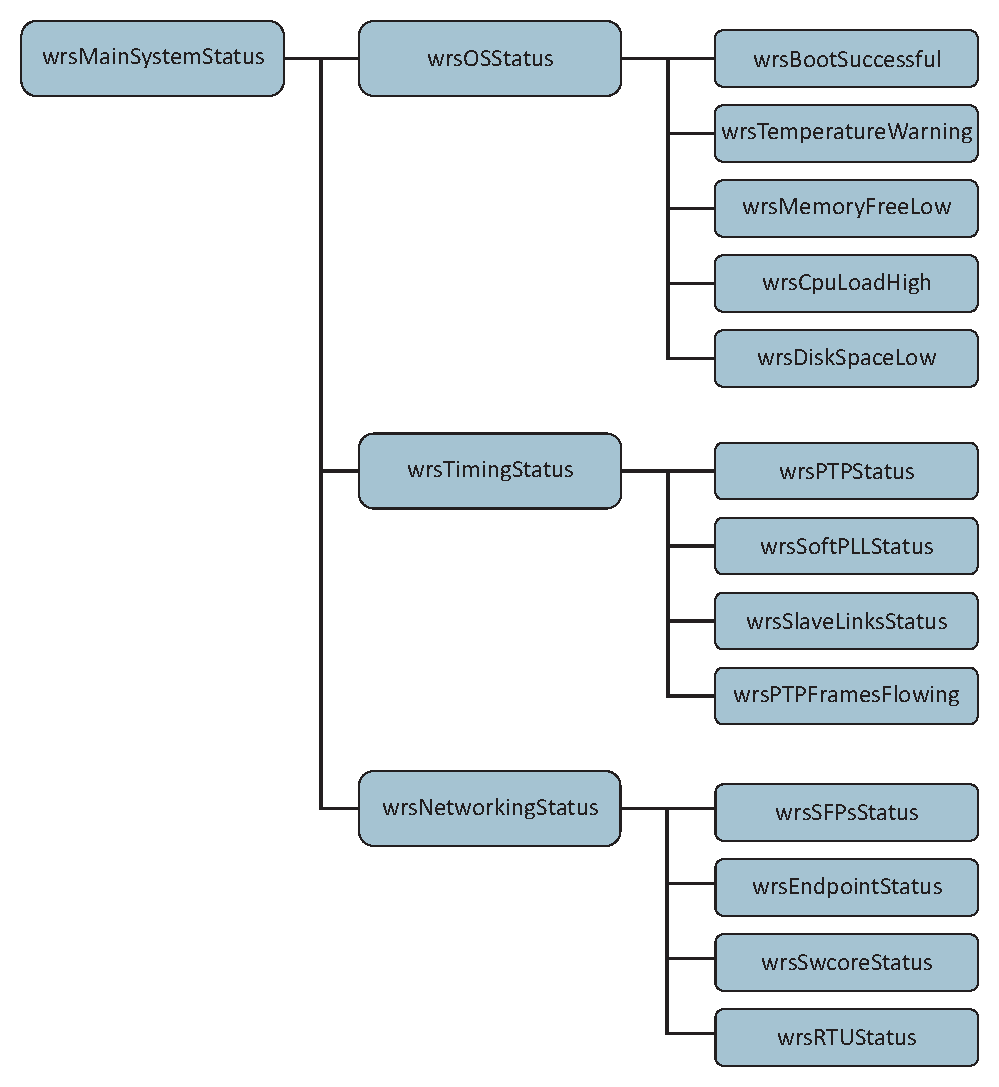
\includegraphics[width=.8\textwidth]{img/snmp_obj.pdf}
    \caption{The structure of general status objects for operators}
    \label{fig:snmp_oper}
  \end{center}
\end{figure}
\begin{itemize}%[leftmargin=0pt]
  \item \texttt{NA} -- status value was not calculated at all (returned value
    is 0). Something bad has happened.
  \item \texttt{OK} -- status of the particular object is correct.
  \item \texttt{Warning} -- objects used to calculate this value are outside the
    proper values, but problem in not critical enough to report \texttt{Error}.
  \item \texttt{WarningNA} -- at least one of the objects used to calculate the
    status has a value \texttt{NA} or \texttt{WarningNA}.
  \item \texttt{Error} -- error in values used to calculate the particular
    object.
  \item \texttt{FirstRead} -- the value of the object cannot be calculated
    because at least one condition uses deltas between the current and previous
    value. This value should appear only at first SNMP read. Threated as a
    correct value.
  \item \texttt{Bug} -- Something wrong has happened while calculating the
    object. If you see this please report to WR developers.
\end{itemize}

\paragraph*{SNMP objects:}

% SNMP status objects
\printnoidxglossary[type=snmp_status,title=,style=objtree,sort=def]

\newpage
\subsection{Expert objects}
\label{sec:snmp_exports:expert}

\paragraph*{SNMP objects:}
% SNMP expert objects
\printnoidxglossary[type=snmp_expert,style=objtree,sort=def]

\vspace{12pt}
\paragraph*{Objects from other MIBs:}
% other objects
\printnoidxglossary[type=snmp_other,style=objtree,sort=def]

%%%%%%%%%%%%%%%%%%5
%% Other notes
%
% What else should be reported in the future
% Status of Primary Slave port and backup links
% For backup timing links, report parameters from Backup SPLL channels and PTP servo
% What can be reported regarding eRSTP ?
% %	role of the bridge - root/designated
% % port role - root/designated/backup/alternate/disabled
% % number of exchanged BPDUs
%
% * we could use information from RSTP to visualize the topology of network made of switches
% * switches exchange BPDU messages to leard about other switches
% * RFC 2674 - Bridges with priority, multicast pruning and VLAN

%\section{SNMP exports}
%\subsection{Operator/basic objects}
%\subsection{Expert objects}

%\newpage
%\bibliographystyle{unsrt}
%\bibliography{references}

\end{document}
